\documentclass[aspectratio=169,11pt,hyperref={colorlinks=true}]{beamer}
\usepackage[utf8]{inputenc}
\usepackage[T1]{fontenc}
\usepackage{fontspec}
\usepackage[absolute,overlay]{textpos}
\usepackage{listingsutf8}
\usepackage{listings-golang}
\usepackage{tikz}
\usepackage{color}


\title{Tekton 101}
\date[kubeconna2019]{November 19th 2019}
\author[Andrea]{%
  Andrea Frittoli \\
  Open Source Developer Advocate \\
  andrea.frittoli@uk.ibm.com \\
  @blackchip76
}
\institute[kubeconna2019]{%
  KubeCon and CloudNativeCon North America 2019
}

\usetheme{ibmcloud}

% Code style
\setlststyle

\lstdefinelanguage{koyaml}{
  keywords={github, com, afrittoli, examples, ms, go, helloworld},
  sensitive=false,
  comment=[l]{\#},
  morestring=[b]',
  morestring=[b]"
}

% Automatic section frame
\AtBeginSection{\frame{\sectionpage}}

\begin{document}

\begin{frame}[noframenumbering]
\titlepage{}
\end{frame}

% The main points of the talk are (TBD):
% - Give an introduction to Tekton Pipelines
% - Get in some more details with an example
% - Talk about Kaniko and source to image with tricky bits
% - Reusing tasks, dev vs CI vs CD
% - can I use Tekton? Where? security concerns

% The slide/section order does not match the narrative yet

%% TBD

\section{A Bit of History}

\begin{lblackrwhiteframe}
  \frametitle{Knative}
  \large
  \begin{beamercolorbox}[wd=0.3\paperwidth]{text}
    \begin{itemize}
      \item Beginning of 2018...
      \item Knative:
      \begin{itemize}
        \item Build
        \item Eventing
        \item Serving
      \end{itemize}
    \end{itemize}
    \begin{itemize}
      \item OpenSource
      \item Contributors:
      \begin{itemize}
        \item Google
        \item Pivotal
        \item IBM
        \item RedHat
        \item Cloudbees
        \item ...and others
      \end{itemize}
    \end{itemize}
  \end{beamercolorbox}%
  \begin{textblock*}{0.5\paperwidth}(0.5\paperwidth,0.2\paperheight)
    \centering
    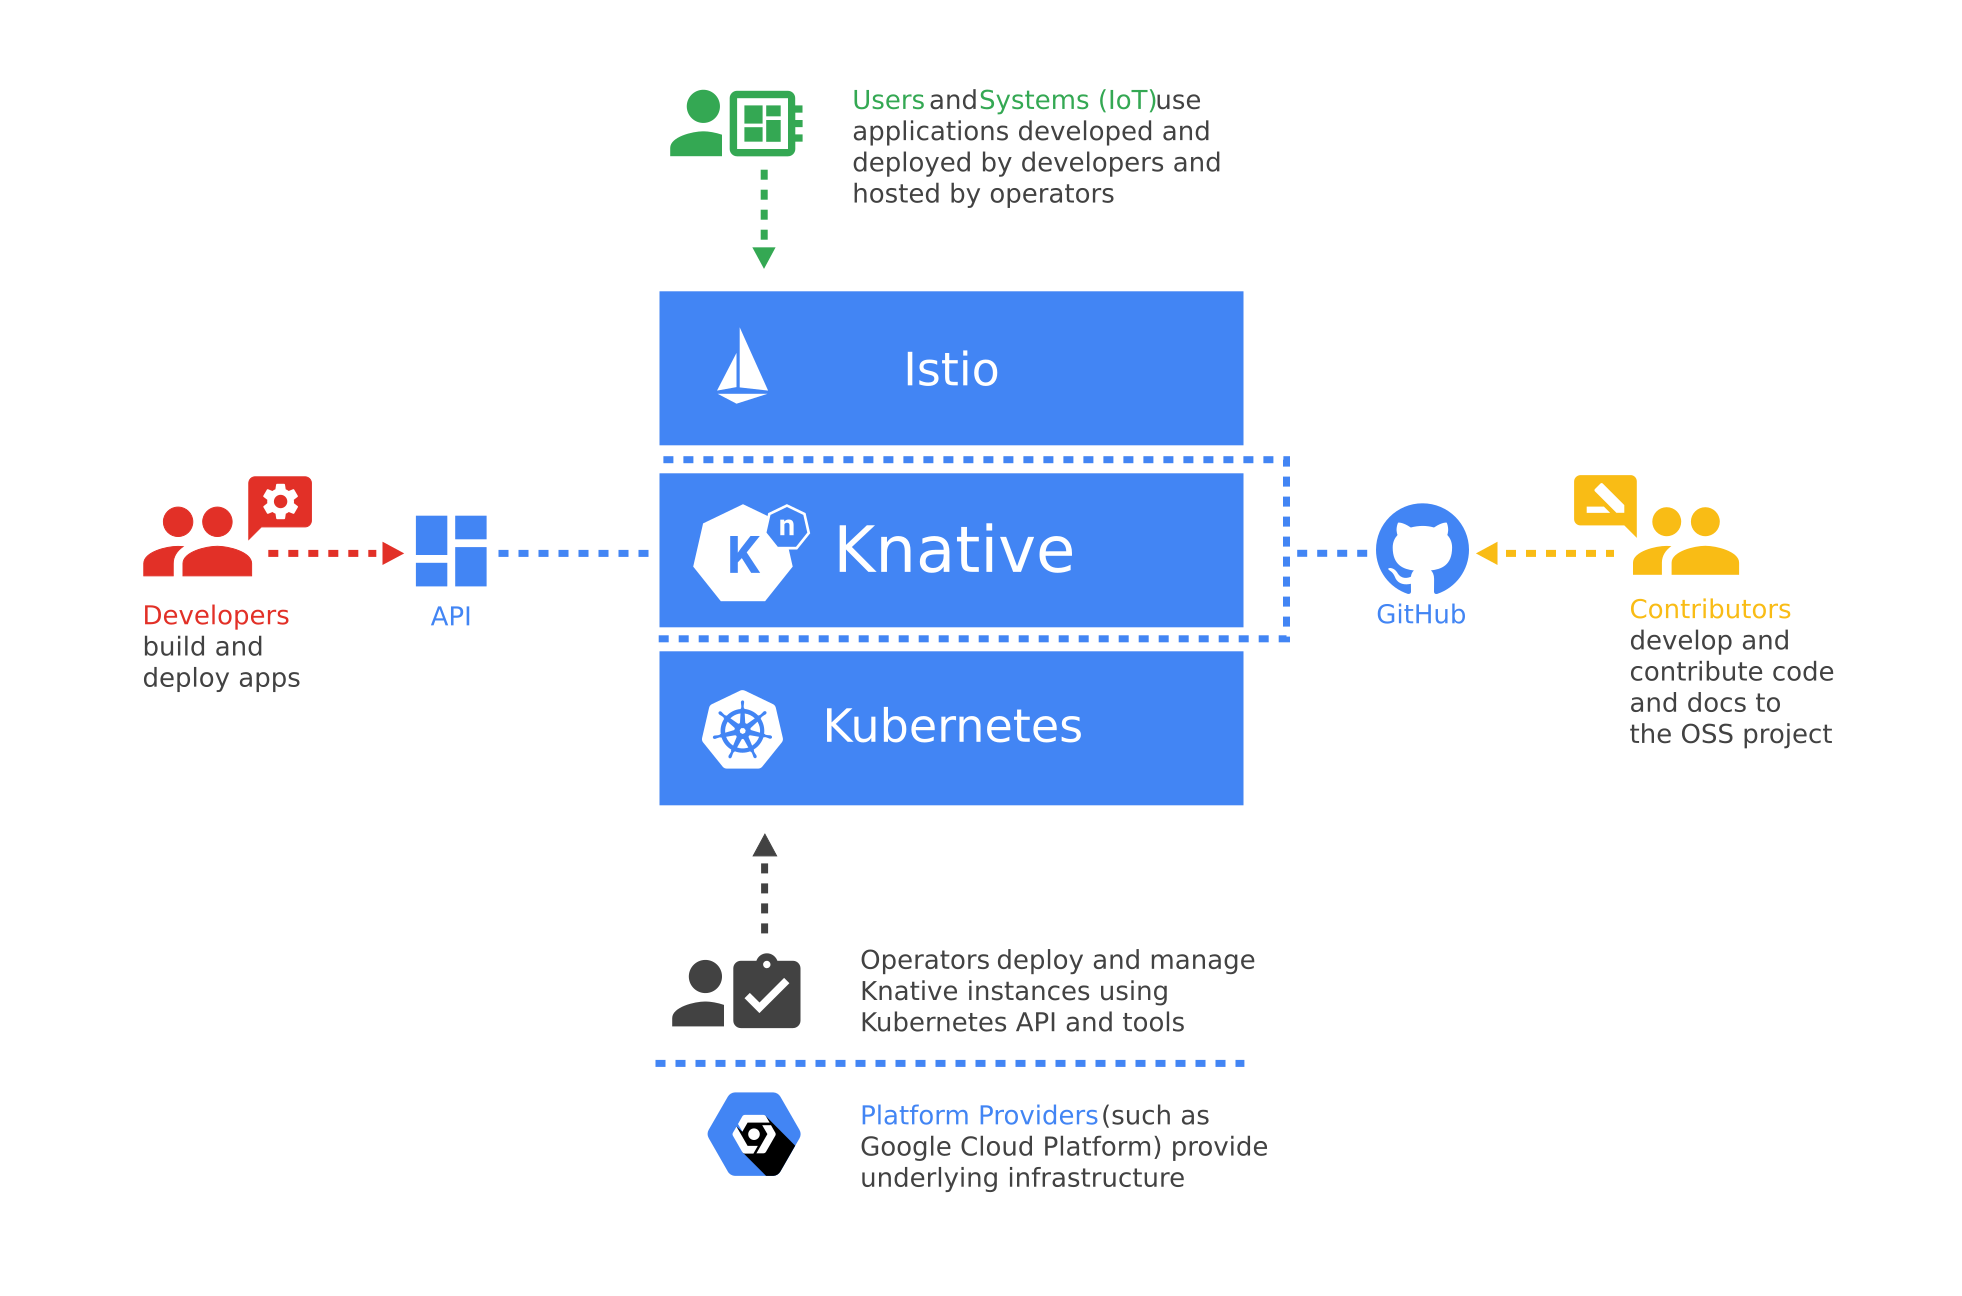
\includegraphics[width=0.45\paperwidth]{img/knative-audience.png}
  \end{textblock*}
\end{grayframe}

\begin{grayframe}
  \frametitle{Community}
  \begin{itemize}
    \item Steering Commitee (SC)
    \item Technical Oversight Commitee (TOC)
    \item Dedicated Working Groups (WG)
    \item Various Contribution profiles
    \item Design, issues: on GitHub
    \item Communication:
    \begin{itemize}
      \item WG periodic meetings, recorded
      \item Asynch: Knative Users / Developers ML
      \item Sync: slack.knative.dev
    \end{itemize}
  \end{itemize}
\end{grayframe}

\begin{tblackbgrayframe}
  \frametitle{Going further}
  \begin{textblock*}{0.75\paperwidth}(0.15\paperwidth,0.25\paperheight)
    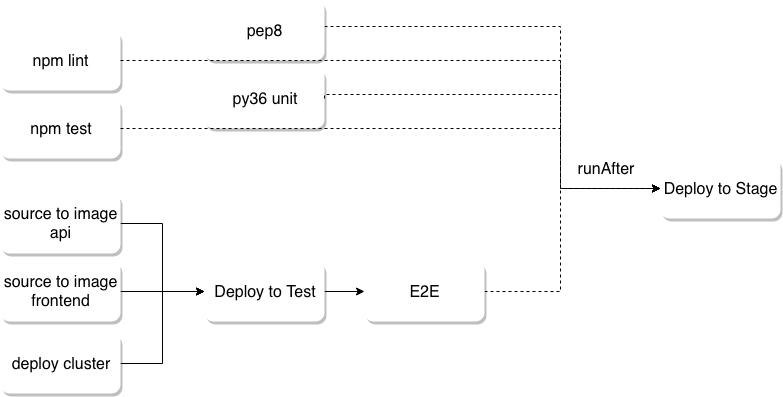
\includegraphics[width=0.75\paperwidth]{img/test-pipeline.png}
  \end{textblock*}
\end{tblackbgrayframe}

\begin{blackframe}
  \frametitle{\textasciitilde Sept 2018: Knative Pipelines}
  \begin{textblock*}{\paperwidth}(0cm,0.2\paperheight)
    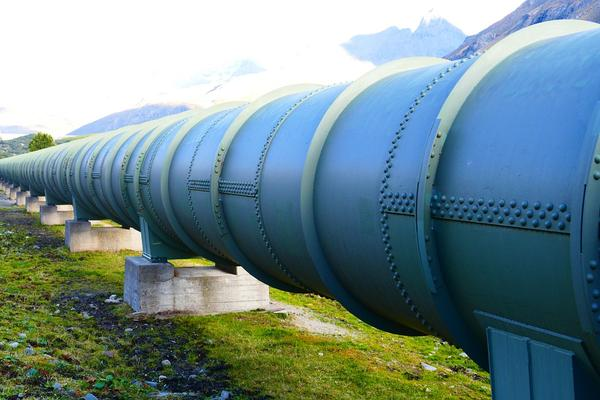
\includegraphics[width=\paperwidth]{img/pipeline_cc0.jpg}
    % https://mediad.publicbroadcasting.net/p/shared/npr/styles/placed_wide/nprshared/201804/605180710.jpg
  \end{textblock*}
  \begin{textblock*}{0.2\paperwidth}(0.83\paperwidth,0.93\paperheight)
    
\includegraphics[width=0.03\paperwidth]{img/cc.png}
    
\includegraphics[width=0.03\paperwidth]{img/zero.png}
  \end{textblock*}
\end{blackframe}

\begin{lblackrwhiteframe}
  \frametitle{Latest news!}
  \large
  \begin{beamercolorbox}[wd=0.35\paperwidth]{text}
    \begin{itemize}
      \item Tekton pipelines (March 2019)
      \item Focus on CI/CD
      \item @CD Foundation  (March 2019)
      \item Deploy ``anywhere''
      \item Replaces Knative Build (June 2019)
      \item Bootstrap governance
    \end{itemize}
  \end{beamercolorbox}%
  \begin{textblock*}{0.5\paperwidth}(0.5\paperwidth,0.25\paperheight)
    \centering
    
\includegraphics[width=0.35\paperwidth]{img/tekton-horizontal-color.png}
    
\includegraphics[width=0.20\paperwidth]{img/cdf-color.png}
  \end{textblock*}
\end{lblackrwhiteframe}

\section{Tekton Pipelines}

\begin{blackframe}
  \frametitle{Cloud Native Pipelines}
  % Cloud Native Pipelines, run on Kubernetes
  \begin{textblock*}{\paperwidth}(0.05\paperwidth,0.2\paperheight)
    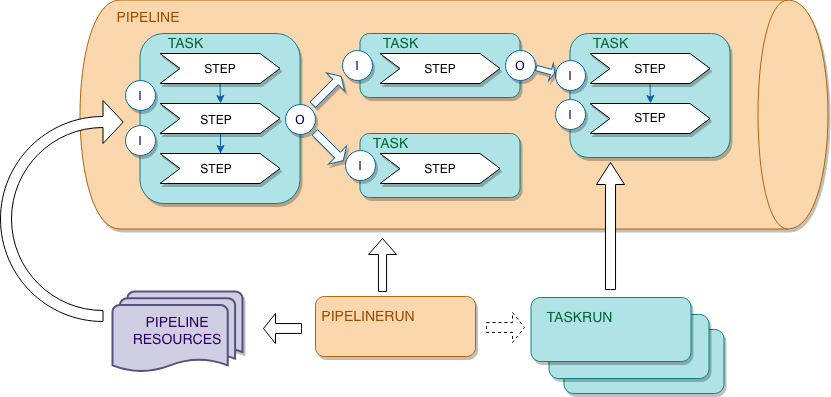
\includegraphics[width=0.85\paperwidth]{img/tekton.png}
  \end{textblock*}
  \begin{textblock*}{0.2\paperwidth}(0.9\paperwidth,0.83\paperheight)
    
\includegraphics[width=0.03\paperwidth]{img/cc.png}
    
\includegraphics[width=0.03\paperwidth]{img/zero.png}
  \end{textblock*}
\end{grayframe}

\begin{2columnsframe}
  {
    \begin{itemize}
      \item Steps are sequential
      \item Tasks are a Directed Acyclic Graph
      \item Order defined by:
      \begin{itemize}
        \item {\em from}: input / output
        \item {\em runAfter}: enforced ordering
      \end{itemize}
    \end{itemize}
  }
  % Graph of a CD pipeline
  {
  \begin{textblock*}{0.65\paperwidth}(0.30\paperwidth,0.30\paperheight)
    \centering
    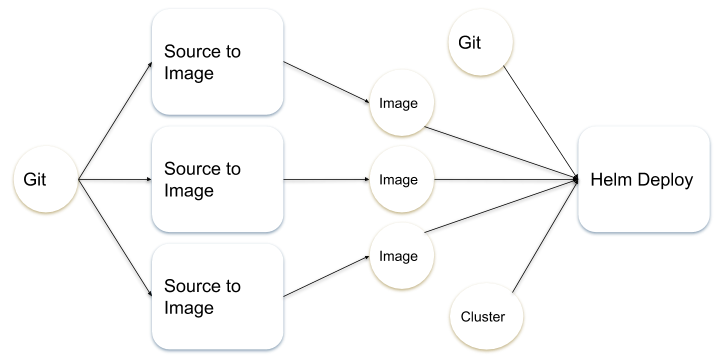
\includegraphics[width=0.65\paperwidth]{img/pipeline.png}
  \end{textblock*}
  }
  \frametitle{Sample pipeline}
\end{2columnsframe}

\begin{2columnsframe}
  {
  {\tiny Source to Image (spec only): \\}
  \lstinputlisting[language=koyaml,firstline=6,lastline=31]{code/task-source-to-image.yaml}
  }
  {
  \lstinputlisting[language=koyaml,firstline=32,lastline=55]{code/task-source-to-image.yaml}
  % {\tiny Cache Warmer (spec only): \\}
  % \lstinputlisting[language=koyaml,firstline=21,lastline=35]{code/task-kaniko-cache.yaml}
  }
  \frametitle{Sample Task: Source to Image}
\end{2columnsframe}

\begin{2columnsframe}
  {
  \begin{itemize}
    \item Pipeline and Tasks:
    \begin{itemize}
      \item Static definition, stored in git
    \end{itemize}
    \item PipelineRuns and TaskRuns:
    \begin{itemize}
      \item Specific to one execution
      \item Generated programmatically
    \end{itemize}
    \item Parameters and Resources:
    \begin{itemize}
      \item Env / run specific
    \end{itemize}
  \end{itemize}
  \vspace{0.3ex}
  \lstinputlisting[language=koyaml]{code/resource-git.yaml}
  }
  {
  \lstinputlisting[language=koyaml]{code/resource-cluster.yaml}
  \vspace{0.3ex}
  \lstinputlisting[language=koyaml]{code/resource-image.yaml}
  }
  \frametitle{Pipeline as code}
\end{2columnsframe}

\section{Tekton Projects}

\begin{2columnsframe}
  {
  \begin{itemize}
    \item Pipeline
    \item Dashboard
    \item CLI
    \item Catalog
    \item Trigger
    \item Plumbing
  \end{itemize}
  }
  {
  \begin{itemize}
    \item Operator
    \item Community
    \item Friends
    \item Website (https://tekton.dev/)
  \end{itemize}
  }
  \frametitle{All Tekton projects}
\end{2columnsframe}

\begin{grayframe}
  \frametitle{References}
  \begin{itemize}
    \item This Talk: https://github.com/afrittoli/tekton\_pipelines\_knative\_intro/tree/oss-jp-2019
    \item Tekton Links:
    \begin{itemize}
      \item https://tekton.dev/, https://cd.foundation/
      \item https://github.com/tektoncd/pipeline
      \item https://github.com/tektoncd/pipeline
      \item https://github.com/tektoncd/pipeline/blob/master/api\_compatibility\_policy.md
      \item https://github.com/tektoncd/pipeline/blob/master/roadmap-2019.md
    \end{itemize}
    \item Knative Community: https://github.com/knative/docs/tree/master/community
    \item Kaniko: https://github.com/GoogleContainerTools/kaniko
    \item Source code and my blog:
    \begin{itemize}
      \item https://github.com/afrittoli/health-helm/tree/knative
      \item https://github.com/afrittoli/openstack-health/tree/knative-eventing
      \item https://github.com/afrittoli/github\_tekton\_glue
      \item https://andreafrittoli.me
    \end{itemize}
    \item IBM Cloud: https://cloud.ibm.com
  \end{itemize}
\end{grayframe}

\section{Q\&A}

\end{document}
